\section{The Socio-Economics of Lifelong Learning}
\shorttitle{Socio-economics of Lifelong Learning}

We define socio-economic research on lifelong learning as the combination of economic research, for example human capital formation and accumulation, with the sociological research of social processes. Market failure in the provision and investment in lifelong learning is our starting hypothesis. Our research group studies ``critical'' transitions over the life course and analyses the medium term impact of transitions on learning and employment careers. The life course perspective provides the central analytical tool, which allows us to study individual trajectories and the evolution of societies as a whole. 

 Our research focuses on (1) processes of social stratification as they are co-determined by learning processes for adults, (2) the sociology of education as the involvement of specific groups like migrants is concerned and (3) the ageing of the work force and implications for lifelong learning. Each of these fields is approached with an emphasis on the links between working and learning in modern societies as they concern individuals, households, firms and whole country systems. 

 We study transitions throughout the life course, which range from labor market entry, reentry after career breaks to gradual retirement with special attention on implications for aging societies. These social dynamics are modeled by use of a transition theory that is based on notions of coupled oscillations (Sch\"{o}mann and O'Connel 2002) and synchronization techniques, which are derived from dynamic systems theory. The rising importance of work-related lifelong learning in non-formal settings is studied through the comparisons of successful combinations of learning and working in firms and comparisons across the European Union. 

 Currently co-financed research projects deal with socioeconomic aspects of lifelong learning in two major areas: (1) lifelong learning and the labor market as well as (2) implications of ageing work forces for learning and working.

\subsection{Lifelong Learning and the Labor Market}


\index{Sch\"{o}mann, Klaus}

\paragraph{Research Team}
Klaus Sch\"{o}mann (Professor), Anette Fasang (Doctoral Fellow), Sara-Izabella Geerdes (Doctoral Fellow), Liuben Siarov (Research Associate), Christoph Hilbert (Doctoral Fellow, Wissenschaftszentrum Berlin f\"{u}r Sozialforschung).

 Research in this area analyzes the links between lifelong learning and the labor market. We analyze sources of market failure, such as multiple factors responsible for underinvestment in lifelong learning. Persistent imbalances in supply and demand for training lead to a lack of participation in further training. In human capital theory, workers will invest until the marginal increase in wages equals the marginal cost of training. However, frequently there is no direct link between further training and returns to training (i.e., increase in wages or productivity) and workers therefore hesitate to take time out from the labor market to invest in training. The overdue change in reversing an ``early retirement culture'' in many European countries makes investment at later stages of the life course more attractive to employers and employees due to longer periods of returns on investments.

 Risk aversion and budgetary constraints in form of access to loans for purposes of learning also explain why people are reluctant to participate in training. Additionally firms might fear ``poaching'' of training costs of employees by other firms, although this problem can be addressed by adequate contractual arrangements.

 Further ways of tackling the barriers to participation in training are ensuring access to loans, promoting information availability, promoting transparency in training, certification and recognition of professional experience, targeting the groups least likely to participate by lifelong learning policies, the low-qualified and older workers. Research in these fields makes use secondary data analysis like panel data, large European surveys or own data collection through lab 3 resources like computer assisted telephone interviews. 

\textbf{Research Highlights 2006}

 Recent findings show that there are effective policies to reduce stigmatization of older workers and to combat the notion that older workers are less able or less willing to learn. Hence it is not only important to increase the budgets involved, but rather tackle the stigma that older people are less interested in learning. This complements the findings from the other disciplines, mainly psychology, in this area (see above).

 Drawing on the argument that lifelong learning provides mutual benefits to individuals, firms and society as a whole, innovative ways to co-finance lifelong learning are particularly promising policy solutions.

 Recently, we have started to investigate the ``function of learning in geographic and job mobility'' using the Eurobarometer 2005. This project is co-financed by the European Foundation for the improvement of living and working conditions based in Dublin. Our analyses show that skill development is an important element in the process of job mobility. Persons with higher investment in further training seem to be more mobile in the labor market and geographical mobility even across borders is highly linked to further training. The major driving force for participation in training over the last 12 months in the European Union, however, is a person's training initiated upon the employers' request (see Figure \ref{fig1:profKlausSchoemann}). A more proactive and self-motivated approach of individuals is needed to achieve high employment  rates also for older workers throughout the European Union. 

 The same European data source allows us to study various dimensions of job satisfaction across member states of the EU. So far we were able to demonstrate that satisfaction with training opportunities is an important element of overall satisfaction with a job and is part of the overarching domain of career prospects and work content as qualitative elements of a job.

\begin{figure}[ht]
  \begin{center}
    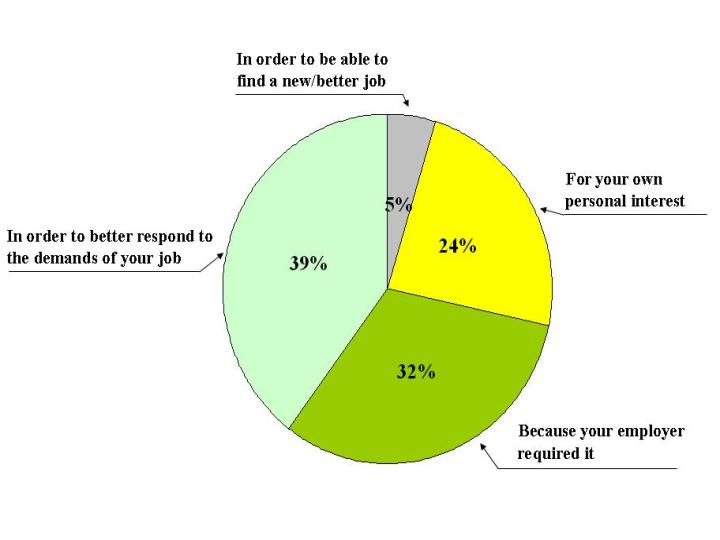
\includegraphics[width=7.5cm]{profKlausSchoemann-fig1.jpg}
    \caption{Reasons for taking part in training, EU 25 (Source: data from the Eurobarometer 2005, own calculations, Geerdes and Sch\"{o}mann 2006).}\label{fig1:profKlausSchoemann}
   \end{center}
\end{figure}

\newpage
\paragraph{Collaborations}
\begin{itemize}
\item Institute for Labour Studies (HIVA) \\ Catholic University Leuven \\ Dr. Tom Vandenberghe (co-ordinator)
\item Institute for Labour Studies (OSA) \\ University of Tilburg \\ Prof. Ruud Muffels 
\item Centre for Labour Market Policy Research (CAFO) \\ V\"axj\"o University \\ Prof. Dominique Anx\"o
\item Economic and Social Research Institute (ESRI), Dublin \\ Prof. Philip O'Connell 
\item Social Economic Research Rotterdam (SEOR) \\ University of Rotterdam \\ Prof. Jaap de Koning
\item Istituto per la Ricerca Sociale (IRS) Roma \\ Dr. Manuela Samek Hugo
\item Hugo Sinzheimer Institute (HSI) \\ University of Amsterdam \\ Prof. Ton Wilthagen; Dr. Els Sol
\item Institut f\"ur H\"ohere Studien (IHS), Wien \\ Prof Dr. Lorenz Lassnigg 
\item MATISSE, Centre National de la Recherche Scientifique, Paris I \\ Prof. Bernard Gazier
\item Institute for Employment Studies (IES) \\ University of Warwick \\ Prof. Ralf Rogowski 
\item McGill University, Canada \\ Prof. Axel van den Berg 
\item Universidad de Alcala, Madrid \\ Prof. Luis Toharia
\item Wissenschaftszentrum Berlin f\"ur Sozialforschung (WZB) \\ Prof. G\"unther Schmid 
\item Centre for Labour Market Research (CARMA) \\ Aalborg University \\ Prof. Per Madsen
\end{itemize}

\begin{bibunit}[apalike]
\nocite{*}
\putbib[profKlausSchoemann]
\end{bibunit}

\paragraph{Grants}

\begin{itemize}
\item European Foundation, 5th Framework Programme of the EU on ``managing social risks through transitional labour markets''. Co-financing by European Commission DG Employment as part of the mutual learning network. The research network consisted of 22 research groups in the European Union and a Canadian partner. The European Foundation in Dublin co-financed the data analysis of the Eurobarometer November 2005 data on labour mobility and geographical mobility in the EU. 
\item BMBF (PI: K. Sch\"omann): Qualification Needs in the OECD - Analysis and Implementation.
\end{itemize}

\subsection{Implications of the Aging Workforce for Learning and Work} 


\index{Sch\"omann, Klaus}

\paragraph{Research Team}
Klaus Sch\"omann (Professor), Anette Fasang (Doctoral Fellow), Paula Aleksandrowicz (Doctoral Fellow).

Germany faces a dual demographic challenge in the next 15 years. This consists in a considerable aging of the working-age population and of the total population, along with a shrinking size of the population of working-age. The size of the working-age population is projected to decline from 50 to 40 million people in 2020. Increasing the participation in employment of older workers is an important consequence of this demographic trend. To enable similar potentials of economic growth in the coming years not only more ``silver workers'' will have to work from each birth cohort, but the extension of the working live becomes likely scenario which is subject of our research interest in the field of productive aging. 

 Our second research theme deals with the links and exchangeability between human capital and social capital. We analyze the potential to increase voluntary work or civic engagement of older workers as the average life expectancy and fitness in older age increase. Thereby we assess the reversibility of retirement transitions and new combinations of market and non-market work in Western societies. 

 The part of sociology in the subproject "Learning" within the framework of the joint BMBF project concerns the area of learning participation and opinions of learning and their match with learning strategies and the learning culture of within a firm under the demographic aging of the employees and management. 

\begin{figure}[h]
  \begin{center}
    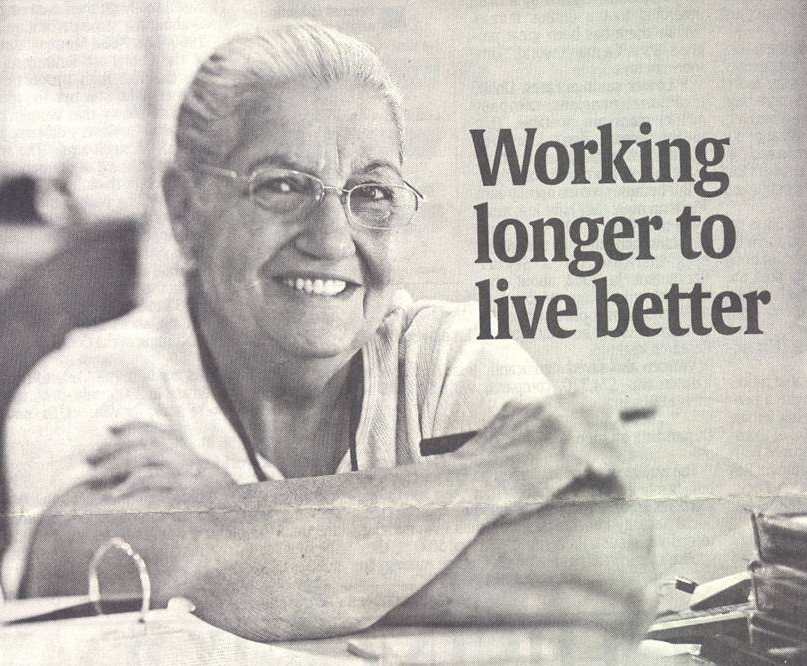
\includegraphics[width=7.5cm]{profKlausSchoemann-fig2.jpg}
    \caption{A challenging research agenda for life course sociology (Source: USA today 14.9.2006).}\label{fig2:profKlausSchoemann}
   \end{center}
\end{figure}

\textbf{Research Highlights 2006}

 Based on our first telephone survey of employees in part-time retirement in one firm we have produced a report on the results for the company executives. We have already achieved a faster turnaround from collecting survey data ourselves to data analysis and publication of results. The finding that even the retirement transition might be a transition, that can be reversed was received with some enthusiasm in the company as they are looking already for means to rehire some of their previous employees sent into early retirement. Similarly the combination of civic engagement of the enterprise and its former employees might constitute an interesting future potential of cooperation beyond the traditional employment relationship of dependent full-time employees in this firm. 

 Additionally we started to cooperate with the ``European initiative for the rights of future generations'' in the field of social policies. 


\paragraph{Collaborations}
\begin{itemize}
\item OECD Department of Employment and Social Affairs
\item Universit\'e Paris I, MATISSE \\ Maitre de Conf\'erences \\ Christine Erhel
\item University of V\"axj\"o  \\ Prof. Dominique Anx\"o 
\item OSA Institute for Labour Studies  \\ Dr. Frank Tros 
\item University of North Carolina at Chapel Hill  \\ Prof. Dr. Arne Kalleberg
\end{itemize}

\begin{bibunit}[apalike]
\nocite{*}
\putbib[profKlausSchoemann2]
\end{bibunit}


\paragraph{Grants}
\begin{itemize}
\item BMBF (PI: JCLL). K. Sch\"omann, C. Ro\ss nagel: subproject ``Learning / Training'' within the joint research project ``Effects of Matches/Mismatches between Aspects of Human and Social Capital, Corporate Strategy and Work Organization on the Physical and Mental Well-Being of Employees''. 
\item Consulting Project (PI: K. Sch\"omann, U. Staudinger): Retirement Processes in a Large Firm.
\item Consulting Project (PI: K. Sch\"omann): Evaluation of company-wide occupational health and safety trainings.
\item Executive Teaching for AutoUni in Wolfsburg by K. Sch\"omann.
\item DFG Travel Grant for Anette Fasang to present her first research results to the Sociology department at Yale, USA.
\item Grant by the European Sociological Association for Sara Geerdes for participation in a Summer School on Migration in Milano, Italy.
\end{itemize}

\subsection{Other Professional Activities}

\begin{itemize}
\item Consultant to OECD, European Commission DG Employment, Brussels and the European Foundation for the Improvement of Living and Working Conditions, Dublin.
\item Administrative Coordinator SISWO (Netherlands, 5th Framework Programme of the European Commission DG Research). 
\end{itemize}

\textit{Editorial Board Membership}

\begin{itemize}
\item Formation Emploi, Revue Fran\c caise de Sciences Sociales (since 2002).
\end{itemize}

 

